\section{Method}
\subsection{Offline and Online Framework}
The proposed system has two stages. In the offline stage, the model is trained on radiographs paired with lesion polygons. Each polygon is converted into a training prompt by generating a simulated bounding box and then transforming that box into a Gaussian-smoothed plateau heatmap. The network learns to map the image-prompt pair to the binary lesion mask. In the online stage, a user provides a coarse bounding box around a suspected lesion on a new radiograph. The same prompt-construction procedure is applied, and the trained model predicts the final lesion mask.

The scientific contribution of this framework is that the prompt is not treated as an optional side input used only at the first layer. Instead, the prompt is encoded as a dense spatial prior and made active at both encoder and decoder stages. The practical consequence is improved robustness when the prompt is coarse, mildly off-center, or applied to a very small lesion.

\subsection{Problem Setting}
Given a grayscale radiograph $\mathbf{I}\in\mathbb{R}^{H\times W}$ and a user-provided bounding box $\mathbf{B}$, the goal is to predict a binary lesion mask $\hat{\mathbf{M}}$. Let $\mathbf{H}(\mathbf{B})$ be the prompt heatmap derived from the box. PGA-UNet predicts
\begin{equation}
\hat{\mathbf{M}} = \mathbf{1}\left[f_{\mathrm{PGA}}\left(\mathbf{I},\mathbf{H}(\mathbf{B});\theta\right)\ge 0.5\right].
\end{equation}

\subsection{Prompt Representation}
The input prompt is not encoded as a hard binary rectangle. Instead, the box interior is converted into a plateau map and its boundaries are softened with Gaussian filtering. In the implementation used for the reported experiments, the box is first assigned a minimum prompt margin before rasterization and then smoothed with a Gaussian kernel. At $256\times256$, the minimum margin is 5 pixels and the kernel size is $31\times31$; at $512\times512$, the corresponding values are 10 pixels and $61\times61$. This preserves the full spatial extent of the region of interest while reducing over-dependence on an abrupt boundary.

During evaluation, prompts are tested in two settings. A covering prompt expands the lesion bounding box by 15\%--45\% of lesion width and height. An off-center prompt first applies the same expansion and then shifts the box by up to 30\% of lesion width and height while still covering the lesion. A single model is trained per dataset and resolution; the prompt condition is varied only at evaluation time unless otherwise stated in the ablation study.

Let $(x_1,y_1,x_2,y_2)$ denote the tight lesion box and let $w=x_2-x_1$ and $h=y_2-y_1$. The simulated covering box expands each side by a random fraction in $[0.15,0.45]$ of $w$ or $h$ during training and by a fixed fraction of 0.30 during evaluation. The off-center box applies the same expansion and then adds a translation bounded by $0.30w$ horizontally and $0.30h$ vertically while preserving lesion coverage. This simulation is not a substitute for radiologist-drawn prompts, but it provides a controlled way to test sensitivity to plausible box variation.

Algorithmically, prompt construction follows four steps: 1) derive a lesion box from the polygon annotation or user input, 2) enlarge that box with a resolution-aware minimum margin, 3) rasterize the enlarged region into a plateau mask, and 4) smooth the plateau boundary with a Gaussian kernel. This sequence avoids the hard-edge dependence of a binary box while preserving a clear spatial prior.

\subsection{Prompt Spatial Gate}
Let $\mathbf{x}^{l}$ denote the encoder feature map at level $l$. PSG modulates it with a prompt-derived attention map $\mathbf{A}^{l}_{\mathrm{PSG}}$:
\begin{equation}
\widetilde{\mathbf{x}}^{l}
=
\mathbf{x}^{l}\odot
\left(1+\alpha^{l}_{\mathrm{PSG}}\mathbf{A}^{l}_{\mathrm{PSG}}\right),
\end{equation}
where $\odot$ is element-wise multiplication and $\alpha^{l}_{\mathrm{PSG}}$ is learnable. In the implementation, $\alpha^{l}_{\mathrm{PSG}}$ is initialized to 0.1 and clamped to $[0,1]$. The residual form keeps the original feature stream available while emphasizing prompt-relevant regions.

\subsection{Conditional Attention Decoder}
CAD extends decoder attention by conditioning the skip gate on prompt-encoded features. Let $\mathbf{g}^{l}$ be the decoder gating feature and $\mathbf{p}^{l}_{\mathrm{enc}}$ the prompt encoding at the same scale. The conditioned gate is
\begin{equation}
\mathbf{g}'^{\,l}=\mathbf{g}^{l}+c^{l}\alpha^{l}_{\mathrm{CAD}}w_{l}\mathbf{p}^{l}_{\mathrm{enc}},
\end{equation}
where $c^{l}$ is a prompt confidence scalar, $\alpha^{l}_{\mathrm{CAD}}$ is learnable, and $w_{l}$ is a fixed depth coefficient. This design helps the decoder remain aligned with the prompt even when the box is not perfectly centered.

The prompt encoder in CAD uses two $3\times3$ convolutions with instance normalization and ReLU. The prompt-confidence scalar $c^{l}$ is produced by global average pooling followed by a $1\times1$ convolution and a sigmoid nonlinearity. The decoder depth coefficients are fixed to $\{1.0,0.7,0.4,0.2\}$ from deep to shallow layers. With feature scale 4, the channel widths are $\{16,32,64,128,256\}$ from the shallowest encoder stage to the bottleneck. The CAD mixing coefficient is parameterized as a sigmoid-transformed scalar and initialized near 0.3.

Taken together, the method can be summarized as follows: 1) preprocess the image and prompt into a common square resolution, 2) encode prompt-relevant spatial priors with PSG in the encoder, 3) propagate prompt-conditioned context through CAD in the decoder, and 4) predict the final binary lesion mask. The scientific meaning of the contribution is that prompt information is both spatially softened and repeatedly reused, rather than being injected once and left to dissipate.

\begin{figure}[t]
\centering
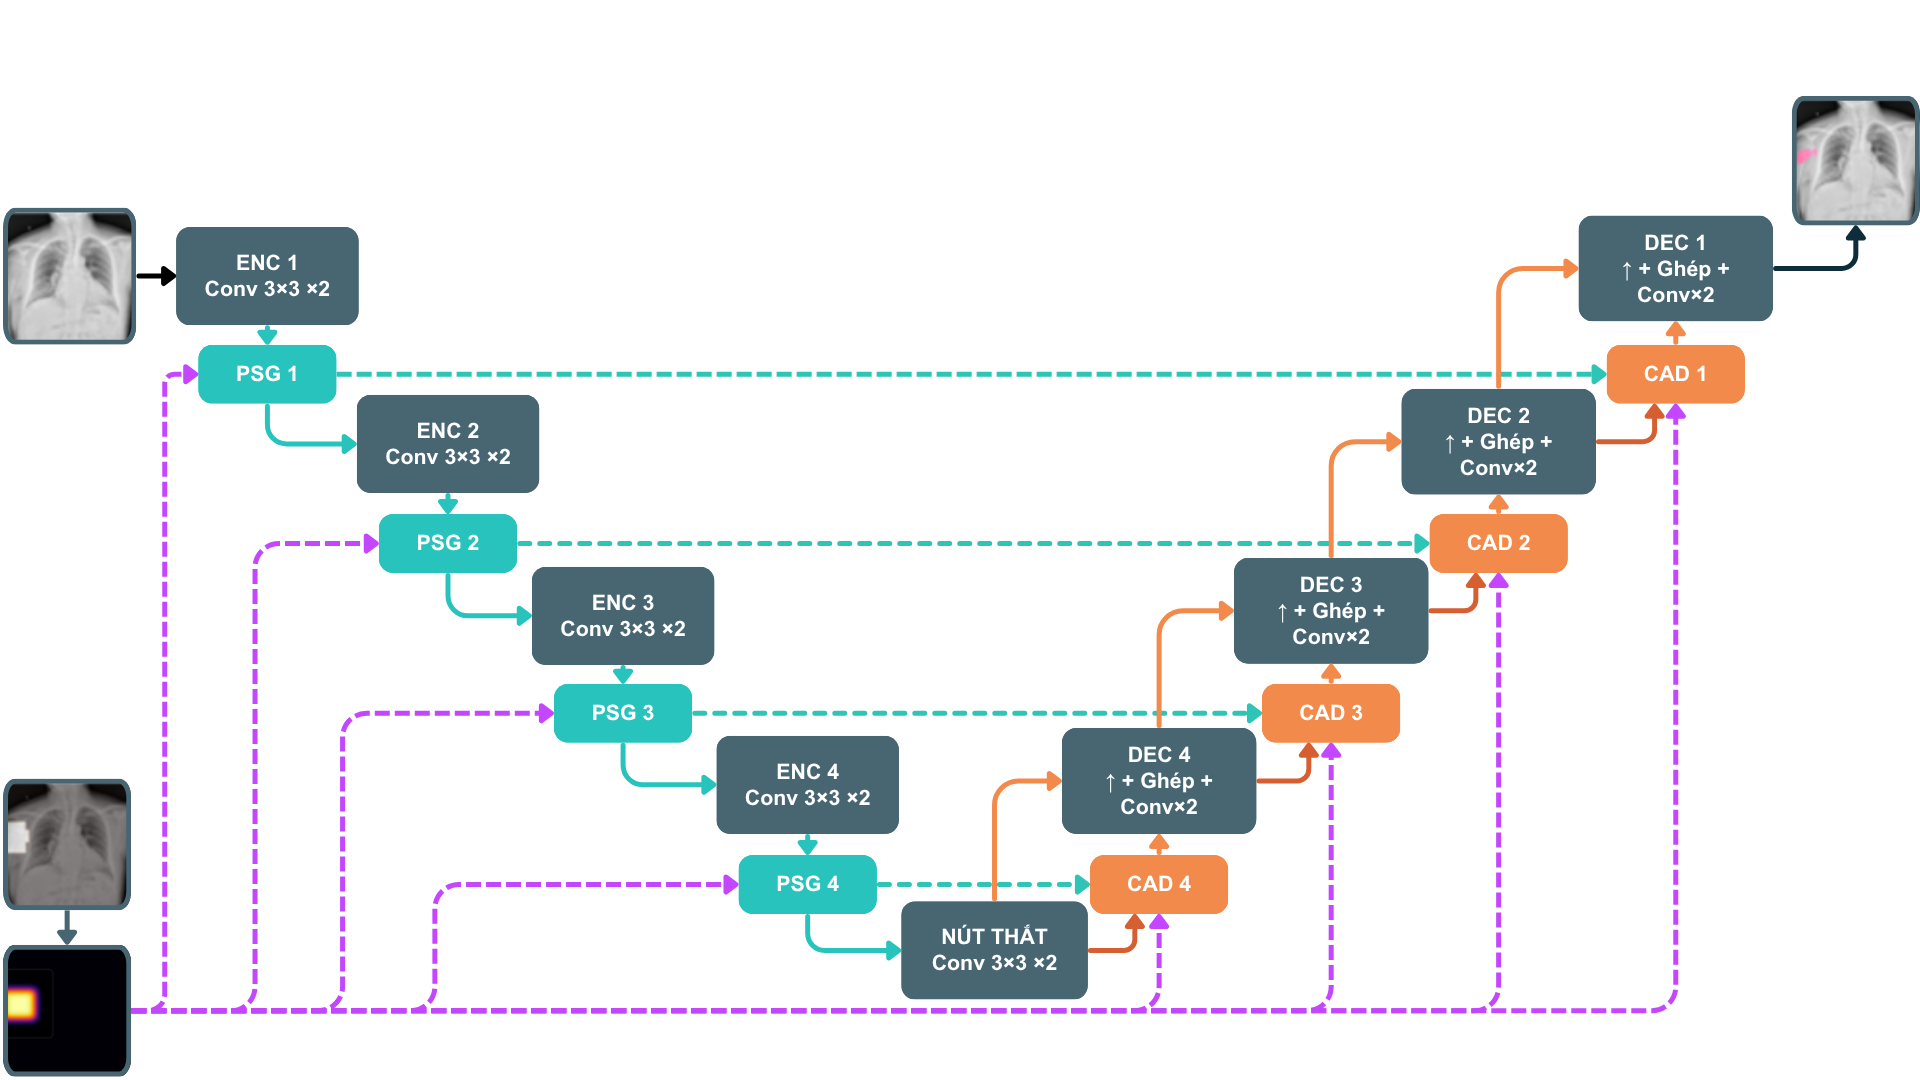
\includegraphics[width=\columnwidth]{images/architecture/architecture_pga_unet.png}
\caption{Overview of PGA-UNet. Prompt information derived from the bounding box is injected into encoder features through PSG and reused in decoder skip attention through CAD.}
\label{fig:arch}
\end{figure}

